\documentclass[10pt,a4paper]{article}
\usepackage[margin=22mm]{geometry}
\usepackage[T1]{fontenc}
\usepackage{lmodern,amsmath,amssymb,graphicx,booktabs,microtype}
\usepackage[font=small,labelfont=bf]{caption}
\usepackage[hidelinks]{hyperref}
\usepackage{fancyhdr}
\pagestyle{fancy}\fancyhf{}
\fancyhead[L]{\small Computational Mechanics Projects}
\fancyhead[R]{\small ShearScope}
\fancyfoot[C]{\thepage}
\setlength{\headheight}{14pt}
\setlength{\parindent}{0pt}\setlength{\parskip}{5pt}
\setlength{\emergencystretch}{1em}
\newcommand{\R}{\mathbb{R}}
\title{\vspace{-1.3cm}\LARGE ShearScope: Diagnosing Shear Locking in Static and Modal Beam Analysis}
\author{\small Computational Mechanics Projects\\\small Reproducible technical research note}
\date{\small 29 September 2026}
\begin{document}\maketitle\thispagestyle{fancy}

\begin{abstract}
Low-order beam elements can produce converged algebraic solutions while severely underpredicting structural compliance. ShearScope isolates this issue by comparing full and selective reduced shear integration in an original two-node Timoshenko element. A C++17 kernel supplies stiffness and consistent mass matrices; Python assembles and solves static and modal problems. An analytical cantilever benchmark and the slender Euler--Bernoulli frequency limit provide independent references. For slenderness $L/h=100$ with eight elements, full integration recovers only 1.96\% of the exact tip compliance, while reduced integration recovers 99.61\%. The study distinguishes discretization locking from equilibrium residuals and states where the validation does not establish physical accuracy.
\end{abstract}
\section{Introduction}
Shear deformation is needed for moderately thick beams, but its discrete representation must also approach the slender bending limit. Linear displacement and rotation fields impose incompatible pointwise constraints when shear strain tends to zero. This creates artificial stiffness, commonly called shear locking~\cite{delft}. The research question is how strongly integration choice alone affects displacement and frequency predictions when geometry, interpolation, material, and loads are otherwise held fixed. The contribution is a reproducible numerical diagnosis rather than a new beam theory.
\section{Mechanical model}
For a straight prismatic beam, let $w(x)$ be transverse displacement and $\theta(x)$ section rotation. Set $A=bh$, $I=bh^3/12$, $G=E/[2(1+\nu)]$, and $S=\kappa GA$, with $\kappa=5/6$. The curvature and shear strain are $\chi=\theta'$ and $\gamma=w'-\theta$. The potential is
\begin{equation}
\Pi=\frac12\int_0^L\!\left[EI(\theta')^2+S(w'-\theta)^2\right]dx
-\int_0^L qw\,dx-Pw(L)-M_t\theta(L).
\end{equation}
With the root fixed, $w(0)=\theta(0)=0$. Defining $V=S(w'-\theta)$ and $M=EI\theta'$ gives $-V'=q$, $-M'-V=0$, $V(L)=P$, and $M(L)=M_t$. Small displacement, elastic response, and uniform properties are assumed. All dimensional examples use SI units.

The kinetic energy includes both translational and rotary inertia:
\begin{equation}
T=\frac12\int_0^L\left[\rho A\dot w^2+\rho I\dot\theta^2\right]dx.
\end{equation}
Consequently the modal problem is $K\phi=\omega^2M\phi$ after constrained degrees of freedom are removed. Frequencies are reported as $\omega/(2\pi)$; mode vectors are normalized in the mass inner product.
\newpage
\section{Discretization and implementation}
For element length $\ell$, the degrees of freedom are $d_e=[w_1,\theta_1,w_2,\theta_2]^T$. With linear shape functions $N_1,N_2$,
\begin{align}
B_b&=[0,-1/\ell,0,1/\ell],& B_s&=[-1/\ell,-N_1,1/\ell,-N_2],\\
K_e&=\int_0^\ell\left(EI B_b^TB_b+S B_s^TB_s\right)dx.
\end{align}
Two-point Gauss integration evaluates the shear contribution exactly for the polynomial integrand; the alternative samples it only at the midpoint. Bending is exact in both variants. Pointwise zero shear requires a constant $w'$ to match a generally linear $\theta$, explaining the overconstraint of full integration in bending. Midpoint integration relaxes this constraint without changing the interpolation.

The consistent mass uses $\ell[\begin{smallmatrix}2&1\\1&2\end{smallmatrix}]/6$ separately for the $\rho A$ and $\rho I$ fields and is never reduced-integrated. The native element API is wrapped with pybind11. Python assembles sparse matrices, eliminates the root constraints, solves $K_{ff}u_f=f_f$, and evaluates reactions and strain energy. A symmetric dense generalized eigensolver computes modes. Element symmetry, rigid-body null modes, mass positivity, and a separately integrated polynomial matrix check the kernel independently of the campaign.
\section{Validation design and results}
The static reference follows directly from the continuum equilibrium equations:
\begin{equation}
w(L)=P\left(\frac{L^3}{3EI}+\frac{L}{S}\right)
+\frac{M_tL^2}{2EI}+q\left(\frac{L^4}{8EI}+\frac{L^2}{2S}\right).
\end{equation}
The campaign fixes $L=1$ m, $b=0.02$ m, $E=70$ GPa, $\nu=0.3$, and $\rho=2700$ kg/m$^3$, varying $L/h$ from 5 to 1000 and mesh size from 4 to 64 elements. Eighty static cases and ten three-mode eigensolves are recorded. The slender frequency reference is
\begin{equation}
f_j=\frac{\beta_j^2}{2\pi L^2}\sqrt{\frac{EI}{\rho A}},\qquad
\cos\beta_j\cosh\beta_j=-1.
\end{equation}
This is a limiting comparison, not an exact thick-beam Timoshenko solution.
\begin{center}\begin{tabular}{lr}\toprule
Recorded diagnostic & Value\\\midrule
Full tip-deflection ratio, $L/h=100$, 8 elements & 0.0195771\\
Reduced tip-deflection ratio, same case & 0.9960941\\
Maximum relative static algebraic residual & $8.09\times10^{-8}$\\\bottomrule
\end{tabular}\end{center}
The compliance ratios reveal a large discretization error that a small residual alone cannot diagnose. Separate tests cover force, moment, and distributed loading, reactions, energy/work consistency, nonuniform meshes, and second-order convergence.
Figure~\ref{fig:results} visualizes selected recorded diagnostics.
\newpage
\begin{figure}[!ht]\centering
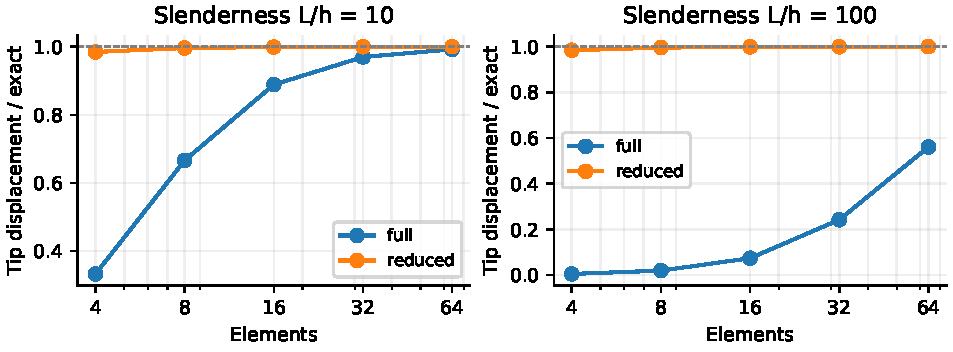
\includegraphics[width=\textwidth]{figure.pdf}
\caption{Recorded tip-compliance convergence at two slenderness ratios. The dashed line is the continuum Timoshenko result. The integration variants share interpolation and mass definitions.}\label{fig:results}\end{figure}
\section{Discussion and limitations}
Selective shear integration substantially improves the slender-beam response in the tested element. This result does not imply that arbitrary underintegrated elements are stable: the element's rank and rigid motions must still be checked. Modal agreement is supported by eigenpair residuals and mass orthogonality, but independently established continuum modal accuracy is restricted to the slender limit.

The model excludes axial load, geometric stiffness, material nonlinearity, damping, and three-dimensional cross-section effects. Unit-load compliance at extreme slenderness may imply deflections outside small-displacement theory; rescaling the load preserves the linear compliance ratio. Very slender or highly graded meshes can be ill-conditioned. Static assembly is limited to 10,000 elements and the dense modal calculation to 500, so the study makes no large-scale performance claim.
\section{Reproducibility and conclusion}
This note documents the committed implementation at \texttt{9345884c87e8} and the existing synthetic results; it does not assert new solver runs. Install from the repository root with \texttt{python -m pip install ".[dev]"}; the README gives compiler requirements and verification commands. Code, data, and this manuscript are available at \href{https://github.com/racostacme-come/shearscope}{the project repository}. No private course material is reproduced. The manuscript was prepared with AI assistance under the project owner\textquotesingle s direction; no peer review is claimed.
The recorded outputs are \texttt{locking.csv}, \texttt{modes.csv}, and \texttt{summary.json} in \texttt{results/}. Reproduce them with \texttt{shearscope campaign --output out}. The principal conclusion is that equilibrium satisfaction and physical approximation quality must be audited separately; varying integration is an effective diagnostic for the particular locking mechanism studied here.
\begin{thebibliography}{9}
\bibitem{delft} TU Delft, \emph{Timoshenko beam: formulation and shear locking}, Computational Modelling textbook. \href{https://teachbooks.tudelft.nl/computational-modelling/structural_linear/timoshenko.html}{Online chapter}.
\bibitem{vibration} S. P. Timoshenko, D. H. Young, and W. Weaver, \emph{Vibration Problems in Engineering}, 4th ed., Wiley, 1974.
\end{thebibliography}

\end{document}
